
% additional usepackage{beamerthemeshadow} is used
\documentclass{beamer}
%\usepackage{beamerthemeshadow}

\usepackage{lmodern} % Font
\usepackage[T1]{fontenc} % Can use danish characters
\usepackage[utf8]{inputenc} %input encoding. Can be used on Linux, Mac and Windows         
\usepackage[english]{babel} %Split words accoding to English

%Standard path to search for pictures
%--------------------------------------------------
%\begin{figure}[hbtp]
%\centering
%\includegraphics[width =0.9 \textwidth]{filnavn-for-png}
%\caption{Titel}
%\label{fig:referenceNavn}
%\end{figure}
%--------------------------------------------------

\usepackage{graphicx}
\usepackage{subcaption}
\usepackage{float}

%Paths the pictures can be located
\graphicspath{
	{../Figures/}
	{Figures/}
}

\begin{document}

\title{Version control and GitHub}  
\author{Rasmus Bækgaard}
\date{\today} 

\frame{\titlepage} 

\frame{\frametitle{Table of contents}\tableofcontents} 


\section{What is version control?} 
\frame{\frametitle{What is version control?} 
\begin{itemize}
\item Why is it needed?
\item When is it needed?
\item Do you need it?
\end{itemize}
}

\subsection{What do you do with files?}
\frame{ 
	\frametitle{What do you do with files?}
\begin{itemize}
\item Create it
\item Save it
\item Modify it
\item Save it again, and again, and again\dots
\end{itemize}
}

\frame{
	\frametitle{How do you save a file only you use?}
	\begin{figure}[hbtp]
	\centering
	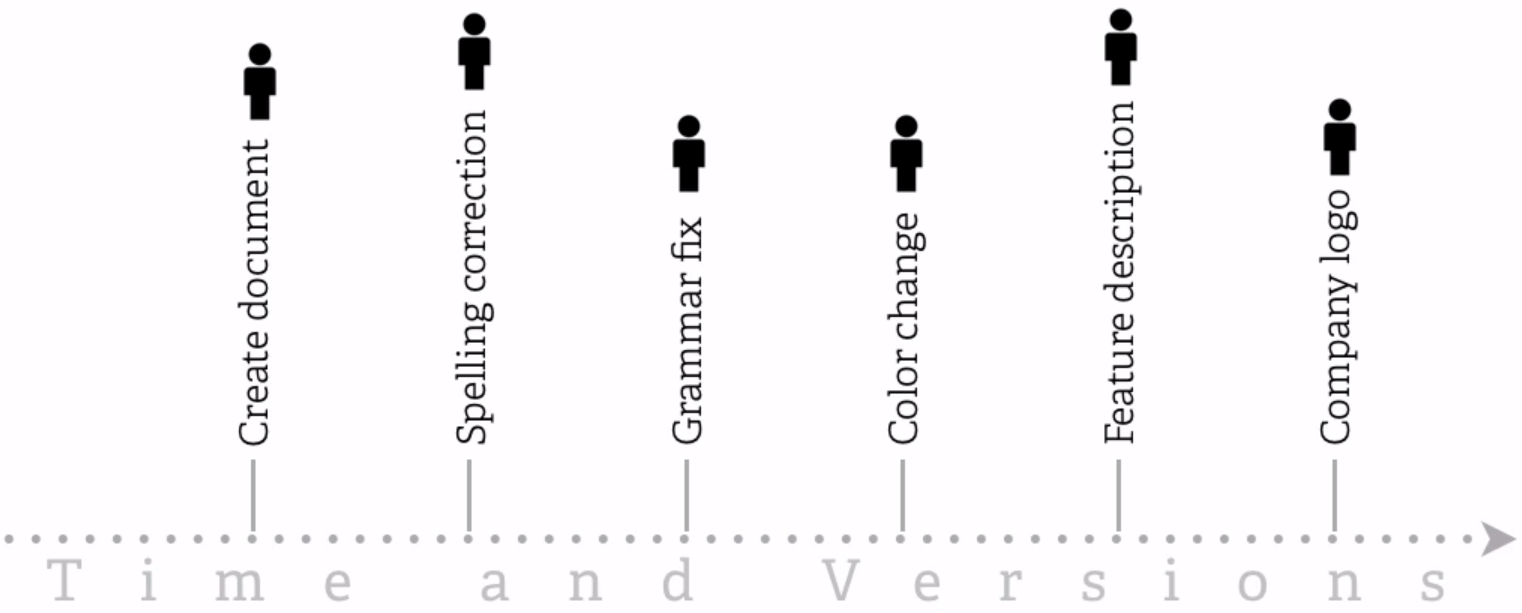
\includegraphics[width=0.9\textwidth]{SingleUser}
	\end{figure}		
}

\subsection{What do you do with files in collaboration?}
\frame{ 
	\frametitle{What do you do with files in collaboration?}
\begin{enumerate}
\item You create it.
\item You save it.
\item Someone modifies it.
\item You modify it.
\item That someone saves it.
\item Now you don't have those changes.
\end{enumerate}
}


\subsection{Merge}
\frame{ 
	\frametitle{Merge}
When conflicts occur they must be solved one way or another.
The most common way is to merge files.
\\
This is taking what was in the original file, the modified, compare them and bring the correct output.
	\begin{figure}[hbtp]
	\centering
	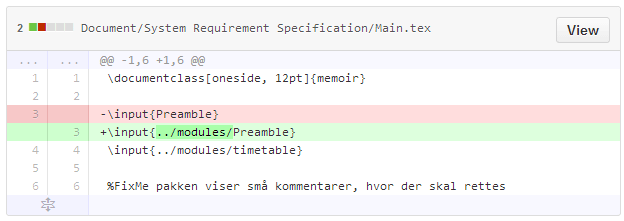
\includegraphics[width=0.95\textwidth]{Merge}
	\end{figure}
}

\section{GitHub} 
\frame{\frametitle{What is GitHub?} 
\begin{itemize}
\item \texttt{Git} was created by Linus Torvals for the Linux kernel because he really didn't like earlier version control systems. 
\item[] If you like others  
	\begin{quotation}
	you are ugly and stupid -- Linus Torvals
	\end{quotation}
\item Bigger projects using it: Android, Perl, Qt, VLC media player etc\dots
\item Will save all the versions of your files and your collaborators versions.
\end{itemize}
}

\subsection{Merge}
\frame{ 
	\frametitle{Merge}
When conflicts occur they must be solved one way or another.
The most common way is to merge files.
\\
This is taking what was in the original file, the modified, compare them and bring the correct output.
	\begin{figure}[hbtp]
	\centering
	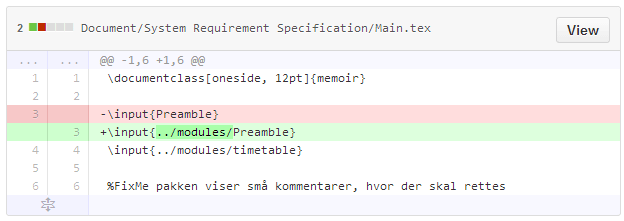
\includegraphics[width=0.95\textwidth]{Merge}
	\end{figure}
}

































\end{document}

